%
% main.tex -- Paper zum Thema <reaktdiff>
%
% (c) 2020 Autor, OST Ostschweizer Fachhochschule
%
% !TEX root = ../../buch.tex
% !TEX encoding = UTF-8
%
\chapter{Reaktionsdiffusionsgleichung\label{chapter:reaktdiff}}
\kopflinks{Thema}
\begin{refsection}
\chapterauthor{Lukas Schöpf}

In diesem Kapitel wird die Reaktionsdiffusionsgleichung
%\cite{reaktdiff:reaktionsdiffwikipedia}
\begin{equation}
\label{reaktdiff:equation:reaktdiff}
\frac{\partial c}{\partial t} = D \Delta c + f(c)
\end{equation}
untersucht.
Sie ist eine nicht lineare partielle Differentialgleichung des zweiten Grades.
Die Reaktionsdiffusionsgleichung beschreibt die zeitliche und Räumliche entwicklung von der grösse \(c\).

\(c(x,t)\) ist ein Vektor und beschreibt die Konzentration eines Stoffes an einem Ort \(x\) zu einem gegebenen Zeitpunkt \(t\).
Die Gleichung \ref{reaktdiff:equation:reaktdiff} besteht aus einem Diffusionsterm und einem Reaktionsterm.
Der Diffusionsterm \(D \Delta c\) beschreibt die räumliche Ausbreitung von \(c\) wobei \(D > 0\) der Diffusionskoefizient eines Stoffes ist.
Der Reaktionsterm \(f(c)\) beschreibt die Reaktion des Stoffes.
Er erlaubt die umwandlung von einem Stoff beschrieben in \(c\) in andere Stoffe.

Der Reaktionsterm kann je nach Anwendung verschiedene Formen annehmen.
Dieses Kapitel wird sich mit verschiedenen Anwendungen der Reaktionsdiffusionsgleichung beschäftigen.
Es werden Anwendung mit einem, zwei oder noch mehr Stoffen betrachtet.
Beginnend wird das Kapitel mit Anwendung bei der \(c\) einen einzenelen Stoff beschreibt.

%
% teil3.tex -- Beispiel-File für Teil 3
%
% (c) 2020 Prof Dr Andreas Müller, Hochschule Rapperswil
%
% !TEX root = ../../buch.tex
% !TEX encoding = UTF-8
%
\section{Gleichungen mit einer Komponente
\label{reaktdiff:section:teil3}}
\kopfrechts{Teil 3}
Die simpleste Reaktionsdiffusionsgleichung ist die welche nur einen Stoff beschreibt.
Die Reaktionsdiffusionsgleichung ist in diesem Fall
\begin{equation}
\label{reaktdiff:equation:fkpp}
\frac{\partial c}{\partial t} = D \frac{\partial^2 c}{\partial x^2} + rc(1-c).
\end{equation}
Um die komplexität zu reduzieren ist \(c\) eindimensional. 
Die Gleichung \ref{reaktdiff:equation:fkpp} ist auch als Fisher-KPP-Gleichung\cite{wikipedia_kpp_fisher} bekannt, benannt nach Roland Fisher, Andery Kolmogorov, Ivan Petrovsky und Nikolai Piskunov.
Sie kann benutzt werden um die Ausbreitung von Populationen zu beschreiben.

\subsection{Mathematische Analyse mti Fourier
\label{reaktdiff:subsection:fkppmathe}}
Aus der Gleichung können die Stationärlösungen abgeleitet werden.
Setzten wir \(\frac{\partial c}{\partial t} = 0\) und \(\Delta c = 0\) erhalten wir die Stationärlösungen
\begin{equation}
\label{reaktdiff:equation:stationaer}
0 = rc(1-c).
\end{equation}
Die Lösungen der Gleichung \ref{reaktdiff:equation:stationaer} sind \(c = 0\) und \(c = 1\).
Um nun das verhalten dieser Lösungen zu untersuchen, fügen wir eine kleine Störung \(\epsilon\) hinzu wobei \(\epsilon \ll 1\).

Für den Fall \(c = 0\) erhalten wir
\begin{equation}
\label{reaktdiff:equation:störung0}
\frac{\partial \epsilon}{\partial t} = D \frac{\partial^2 \epsilon}{\partial x^2} + r\epsilon(1-\epsilon).
\end{equation}
Da \(\epsilon\) sehr klein ist, kann man den Term \(1-\epsilon\) durch \(1\) ersetzen.
Somit wird die Gleichung \ref{reaktdiff:equation:störung0} zu
\begin{equation}
\label{reaktdiff:equation:störung0vereinfach}
\frac{\partial \epsilon}{\partial t} \approx D \frac{\partial^2 \epsilon}{\partial x^2}  + r\epsilon.
\end{equation}
Die Gleichung \ref{reaktdiff:equation:störung0vereinfach} ist eine lineare partielle Differentialgleichung.
Das selbe gilt für den Fall \(c = 1\).
Für den Fall \(c = 1\) erhalten wir
\begin{equation}
\label{reaktdiff:equation:störung1}
\frac{\partial \epsilon}{\partial t} = D \frac{\partial^2 \epsilon}{\partial x^2} - r\epsilon(1-\epsilon).
\end{equation}
Wieder können wir den Term \(1-\epsilon\) durch \(1\) ersetzen.
Somit wird die Gleichung \ref{reaktdiff:equation:störung1} zu
\begin{equation}
\label{reaktdiff:equation:störung1vereinfach}
\frac{\partial \epsilon}{\partial t} \approx D \frac{\partial^2 \epsilon}{\partial x^2} - r\epsilon.
\end{equation}
Die Gleichung \ref{reaktdiff:equation:störung1vereinfach} ist ebenfalls eine lineare partielle Differentialgleichung.
Man sieht das der Unterschied zwischen den beiden Gleichungen \ref{reaktdiff:equation:störung0vereinfach} und \ref{reaktdiff:equation:störung1vereinfach} nur das Vorzeichen des \(r\epsilon\) Term ist.
Um die Gleichungen zu lösen, setzen wir \(\epsilon(x,t) = c_k(t) e^{ikx}\) ein.
Die Ableitungen werden zu
\begin{align*}
\frac{\partial \epsilon}{\partial t} &= \dot{c}_k(t) e^{ikx},\\
\frac{\partial^2 \epsilon}{\partial x^2} &= -k^2 c_k(t) e^{ikx}.
\end{align*}
Setzen wir diese Ableitungen in die Gleichung \ref{reaktdiff:equation:störung0vereinfach} ein, erhält man
\begin{equation}
\label{reaktdiff:equation:störung0vereinfachk}
\dot{c}_k(t) e^{ikx} = -D k^2 c_k(t) e^{ikx} + r c_k(t) e^{ikx}.
\end{equation}
Teilen wir die Gleichung \ref{reaktdiff:equation:störung0vereinfachk} durch \(e^{ikx}\) und \(c_k(t)\) erhalten wir
\begin{equation}
\label{reaktdiff:equation:störung0vereinfachk2}
\dot{c}_k(t) = -D k^2 c_k(t) + r c_k(t).
\end{equation}
Die Gleichung \ref{reaktdiff:equation:störung0vereinfachk2} ist eine gewöhnliche Differentialgleichung.
Die Lösung der Gleichung \ref{reaktdiff:equation:störung0vereinfachk2} ist
\begin{equation}
\label{reaktdiff:equation:störung0vereinfachk3}
c_k(t) = c_k(0) e^{(r - D k^2)t}.
\end{equation}
Setzen wir nun die Gleichung \ref{reaktdiff:equation:störung0vereinfachk3} in die Gleichung \ref{reaktdiff:equation:störung1vereinfach} ein, erhalten wir
\begin{equation}
\label{reaktdiff:equation:störung1vereinfachk}
\dot{c}_k(t) = -D k^2 c_k(t) - r c_k(t).
\end{equation}
Führen wir die selbe Rechnung wie bei der Gleichung \ref{reaktdiff:equation:störung0vereinfachk2} durch, erhalten wir
\begin{equation}
\label{reaktdiff:equation:störung1vereinfachk2}
c_k(t) = c_k(0) e^{(-r - D k^2)t}.
\end{equation}
Aus den beiden Gleichungen \ref{reaktdiff:equation:störung0vereinfachk3} und \ref{reaktdiff:equation:störung1vereinfachk2} können wir die Stabilität der Stationärlösungen \(c = 0\) und \(c = 1\) ablesen.
Unter der Annahmen dass \(D\) und \(r\) immmer positiv sind, ist die Stationärlösungen \(c = 1\) stabil.
Die Stationärlösung \(c = 0\) ist instabil wenn \(r-Dk^2 > 0\) und stabil wenn \(r-Dk^2 < 0\).
Somit werden kleine Störungen um \(c = 0\) wachsen wenn \(k < \sqrt{\frac{r}{D}}\) und abklingen wenn \(k > \sqrt{\frac{r}{D}}\).

Wie bereits erwähnt, ist eine Anwendeung der Fisher-KPP-Gleichung die Ausbreitung von Populationen.
Die Stationärlösungen \(c = 0\) und \(c = 1\) entsprechen dem Fall wo die Population nicht existiert und dem Fall wo die Population die maximale Grösse erreicht hat.
Die Stabilität der Stationärlösungen \(c = 0\) und \(c = 1\) zeigt, dass die Population immer wachsen wird wenn sie klein ist und abklingen wird wenn sie gross ist.

\subsection{Wellenlösung der Fisher-KPP-Gleichung
\label{reaktdiff:subsection:fkppwelle}}
Die Fisher-KPP-Gleichung hat eine Wellenlösung.
Die Wellenlösung ist eine Lösung der Form
\begin{equation}
\label{reaktdiff:equation:fkppwelle}
c(x,t) = C(z), \text{ wobei } z = x - vt,
\end{equation}
wobei \(C\) eine Funktion ist, die die Form der Welle beschreibt und \(v\) die Geschwindigkeit der Welle ist.
Für die Lösung benötigen wir die Ableitungen
\begin{align*}
\frac{\partial c}{\partial t} &= \frac{\partial C}{\partial z}\frac{\partial z}{\partial t} = -vC'(z),
\\
\frac{\partial^2 c}{\partial t^2} &= C''(z).
\end{align*}
Setzen wir die Ableitungen in die Fisher-KPP-Gleichung \ref{reaktdiff:equation:fkpp} ein, erhalten wir
\begin{equation}
\label{reaktdiff:equation:fkppwelle2}
-vC'(z) = D C''(z) + rC(z)(1-C(z)).
\end{equation}
Das ist eine nichtlineare gewöhnliche Differentialgleichung für \(U(z)\)
\begin{equation}
    \label{reaktdiff:equation:fkppwelle3}
    -vC'(z) - D C''(z) - rC(z)(1-C(z)) = 0.
\end{equation}
Für die Analyse untersuchen wir die Gleichung \ref{reaktdiff:equation:fkppwelle3} im Grenzfall \(C(z) \ll 1\).
Um die Gleichung zu lösen, setzen wir \(C(z) = e^{-\lambda z}\) ein.
Somit wird die Gleichung \ref{reaktdiff:equation:fkppwelle3} zu
\begin{equation}
\label{reaktdiff:equation:fkppwelle4}
D\lambda^2 + v\lambda + r = 0.
\end{equation}
Die Lösung der Gleichung \ref{reaktdiff:equation:fkppwelle4} ist
\begin{equation}
\label{reaktdiff:equation:fkppwelle5}
\lambda = \frac{-v \pm \sqrt{v^2 - 4Dr}}{2D}.
\end{equation}
Aus der Gleichung \ref{reaktdiff:equation:fkppwelle5} ist ersichtlich, dass die Welle nur existiert wenn \(v \ge 2\sqrt{rD}\).

\subsection{Numerische Simulation der Fisher-KPP-Gleichung
\label{reaktdiff:subsection:fkppsimulation}}
Die Visualisierung der Fisher-KPP-Gleichung ist unspektakulär.
Die Simulation zeigt eine Welle die sich mit konstanter Geschwindigkeit ausbreitet.
Die Welle hat eine Geschwindigkeit von \(v = 2\sqrt{rD}\).
Denoch regt die Simulation zum Nachdenken an.
Was wäre nun wenn es einen zweiten Stoff gäbe, welches die Reaktion beeinflusst?

\begin{figure}
    \centering
    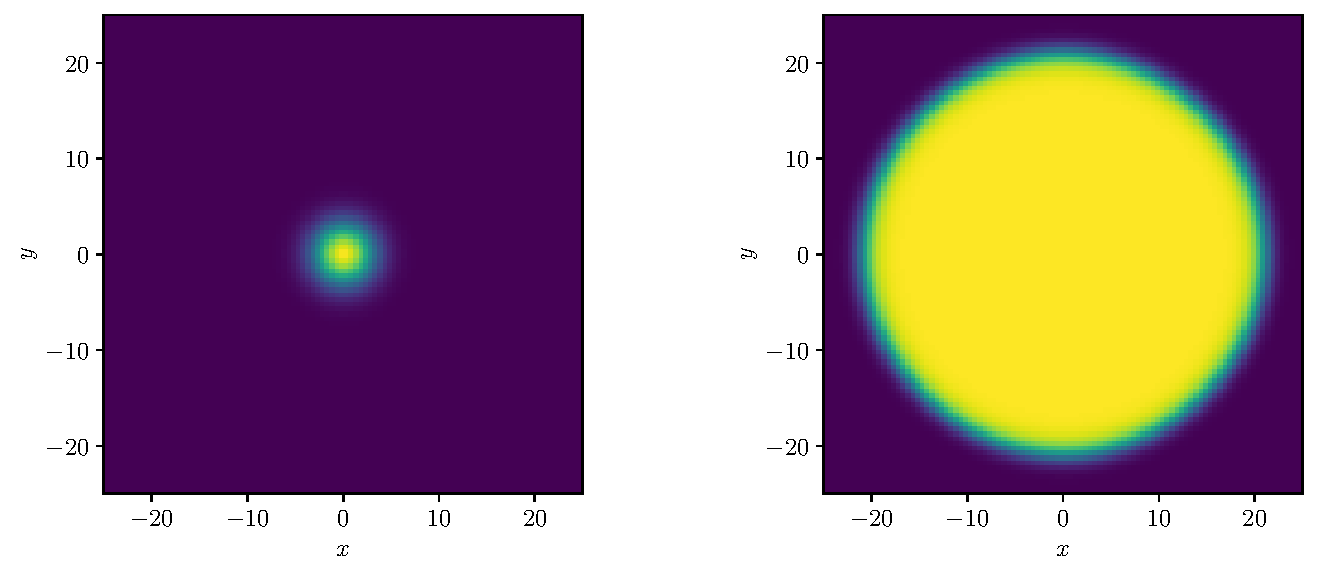
\includegraphics[width=\textwidth]{papers/reaktdiff/images/Fisher_KPP/fisher_kpp_2d_wave_comparison.pdf}
    \caption{Simulation der Fisher-KPP-Gleichung mit \(D = 0.1\) und \(r = 1\). Die Welle breitet sich mit einer Geschwindigkeit von \(v = 0.01\) aus. Das linke Bild zeigt die Simulation zum Zeitpunkt \(t = 0\) und das rechte Bild zum Zeitpunkt \(t = 25\).}
    \label{reaktdiff:figure:fisher_kpp_simulation}
\end{figure}
% %
% einleitung.tex -- Beispiel-File für die Einleitung
%
% (c) 2020 Prof Dr Andreas Müller, Hochschule Rapperswil
%
% !TEX root = ../../buch.tex
% !TEX encoding = UTF-8
%
\section{Einleitung\label{reaktdiff:section:teil0}}
\kopfrechts{Einleitung}





%
% teil1.tex -- Beispiel-File für das Paper
%
% (c) 2020 Prof Dr Andreas Müller, Hochschule Rapperswil
%
% !TEX root = ../../buch.tex
% !TEX encoding = UTF-8
%
\section{Teil 1
\label{reaktdiff:section:teil1}}
\kopfrechts{Problemstellung}
Sed ut perspiciatis unde omnis iste natus error sit voluptatem
accusantium doloremque laudantium, totam rem aperiam, eaque ipsa
quae ab illo inventore veritatis et quasi architecto beatae vitae
dicta sunt explicabo.
Nemo enim ipsam voluptatem quia voluptas sit aspernatur aut odit
aut fugit, sed quia consequuntur magni dolores eos qui ratione
voluptatem sequi nesciunt
\begin{equation}
\int_a^b x^2\, dx
=
\left[ \frac13 x^3 \right]_a^b
=
\frac{b^3-a^3}3.
\label{reaktdiff:equation1}
\end{equation}
Neque porro quisquam est, qui dolorem ipsum quia dolor sit amet,
consectetur, adipisci velit, sed quia non numquam eius modi tempora
incidunt ut labore et dolore magnam aliquam quaerat voluptatem.

Ut enim ad minima veniam, quis nostrum exercitationem ullam corporis
suscipit laboriosam, nisi ut aliquid ex ea commodi consequatur?
Quis autem vel eum iure reprehenderit qui in ea voluptate velit
esse quam nihil molestiae consequatur, vel illum qui dolorem eum
fugiat quo voluptas nulla pariatur?

\subsection{De finibus bonorum et malorum
\label{reaktdiff:subsection:finibus}}
At vero eos et accusamus et iusto odio dignissimos ducimus qui
blanditiis praesentium voluptatum deleniti atque corrupti quos
dolores et quas molestias excepturi sint occaecati cupiditate non
provident, similique sunt in culpa qui officia deserunt mollitia
animi, id est laborum et dolorum fuga \eqref{reaktdiff:equation1}.

Et harum quidem rerum facilis est et expedita distinctio
\ref{reaktdiff:section:teil2}.
Nam libero tempore, cum soluta nobis est eligendi optio cumque nihil
impedit quo minus id quod maxime placeat facere possimus, omnis
voluptas assumenda est, omnis dolor repellendus
\ref{reaktdiff:section:teil3}.
Temporibus autem quibusdam et aut officiis debitis aut rerum
necessitatibus saepe eveniet ut et voluptates repudiandae sint et
molestiae non recusandae.
Itaque earum rerum hic tenetur a sapiente delectus, ut aut reiciendis
voluptatibus maiores alias consequatur aut perferendis doloribus
asperiores repellat.



% %
% teil2.tex -- Beispiel-File für teil2 
%
% (c) 2020 Prof Dr Andreas Müller, Hochschule Rapperswil
%
% !TEX root = ../../buch.tex
% !TEX encoding = UTF-8
%
\section{Teil 2 
\label{reaktdiff:section:teil2}}
\kopfrechts{Teil 2}
Sed ut perspiciatis unde omnis iste natus error sit voluptatem
accusantium doloremque laudantium, totam rem aperiam, eaque ipsa
quae ab illo inventore veritatis et quasi architecto beatae vitae
dicta sunt explicabo. Nemo enim ipsam voluptatem quia voluptas sit
aspernatur aut odit aut fugit, sed quia consequuntur magni dolores
eos qui ratione voluptatem sequi nesciunt. Neque porro quisquam
est, qui dolorem ipsum quia dolor sit amet, consectetur, adipisci
velit, sed quia non numquam eius modi tempora incidunt ut labore
et dolore magnam aliquam quaerat voluptatem. Ut enim ad minima
veniam, quis nostrum exercitationem ullam corporis suscipit laboriosam,
nisi ut aliquid ex ea commodi consequatur? Quis autem vel eum iure
reprehenderit qui in ea voluptate velit esse quam nihil molestiae
consequatur, vel illum qui dolorem eum fugiat quo voluptas nulla
pariatur?

\subsection{De finibus bonorum et malorum
\label{reaktdiff:subsection:bonorum}}
At vero eos et accusamus et iusto odio dignissimos ducimus qui
blanditiis praesentium voluptatum deleniti atque corrupti quos
dolores et quas molestias excepturi sint occaecati cupiditate non
provident, similique sunt in culpa qui officia deserunt mollitia
animi, id est laborum et dolorum fuga. Et harum quidem rerum facilis
est et expedita distinctio. Nam libero tempore, cum soluta nobis
est eligendi optio cumque nihil impedit quo minus id quod maxime
placeat facere possimus, omnis voluptas assumenda est, omnis dolor
repellendus. Temporibus autem quibusdam et aut officiis debitis aut
rerum necessitatibus saepe eveniet ut et voluptates repudiandae
sint et molestiae non recusandae. Itaque earum rerum hic tenetur a
sapiente delectus, ut aut reiciendis voluptatibus maiores alias
consequatur aut perferendis doloribus asperiores repellat.




\printbibliography[heading=subbibliography]
\end{refsection}
